\section*{Anhang}
\label{sec:Anhang}
\addcontentsline{toc}{section}{Anhang}

\begin{figure}
    \centering
    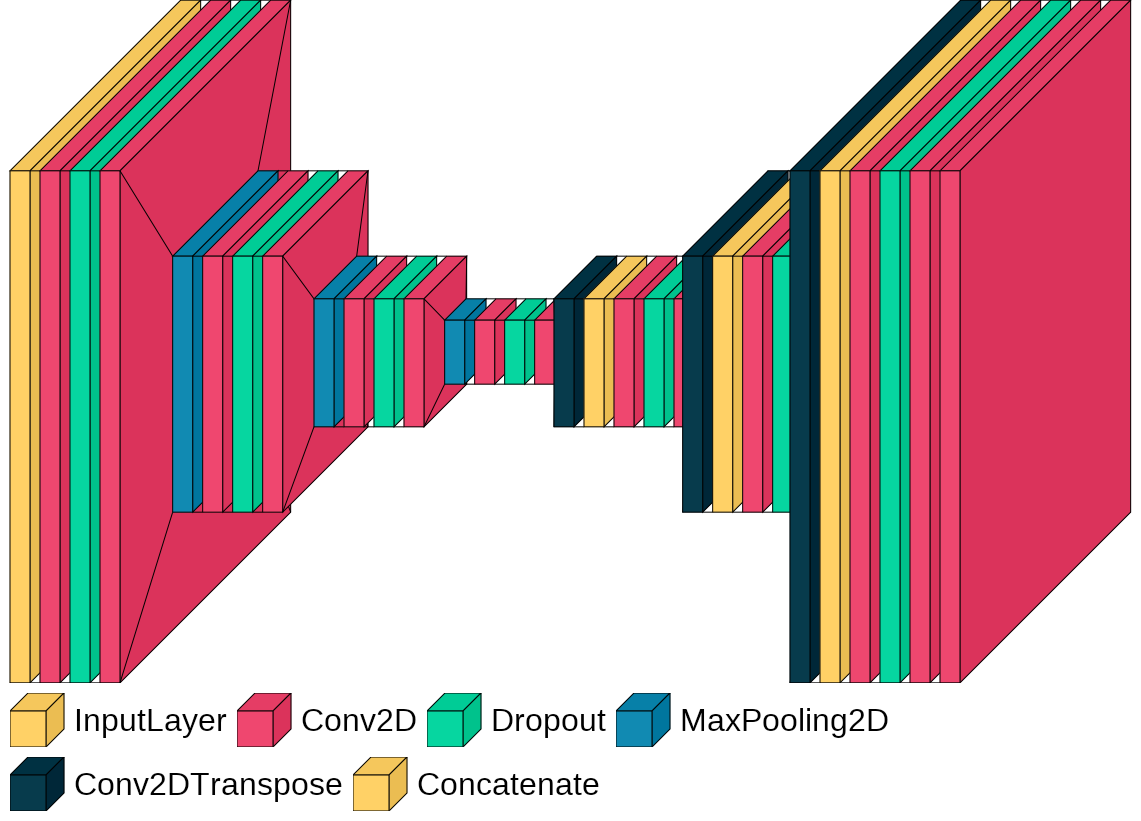
\includegraphics[width=0.6\textwidth]{images/visual_model.png}
    \caption{Visualisierung des verwendeten Convolutional Neural Network.\\%
            Vewendet wurden die folgenden Parameter (von links nach rechts der entsprechenden Lage zugeordnet): \\}
    \label{fig:visual_model}
    \begin{itemize}%
        \item \enquote{InputLayer} Shape: (..., 128, 128, 3) %
        \item \enquote{Conv2D}:%
        \item[-] Filter Anzahl: 18, 18, 36, 36, 72, 72, 144, 144, 72, 72, 36, 36, 18, 18, 1%
        \item[-] Kernel Größe: 3 x 3%
        \item[-] Kernel Initialisierungs-Methode: \enquote{he\_normal}%
        \item[-] Padding: \enquote{same} %
        \item[-] Aktivierungsfunktion: ReLU (letzte: Sigmoid)%
        \item \enquote{Dropout} Stärke: 0.1779, 0.1779, 0.2779, 0.2779, 0.2779, 0.1779, 0.1779%
        \item \enquote{MaxPooling2D} Größe: 2 x 2%
        \item \enquote{Conv2DTranspose}:%
        \item[-] Filter Anzahl: 72, 36, 18%
        \item[-] Kernel Größe: 2 x 2%
        \item[-] Aktivierungsfunktion: keine%
        \item \enquote{Concatenate}: Verkettet Ausgabe vor \enquote{MaxPooling2D} mit Ausgabe nach \enquote{Conv2DTranspose} der gleichen Ebene%
        \item Verlustfunktion: binäre Kreuzentropie%
        \item \enquote{Adam}-Lernrate: 0.003795%
        \item \enquote{Batch}-Größe beim Training: 128%
    \end{itemize}%
\end{figure}

\begin{figure}
    \centering
    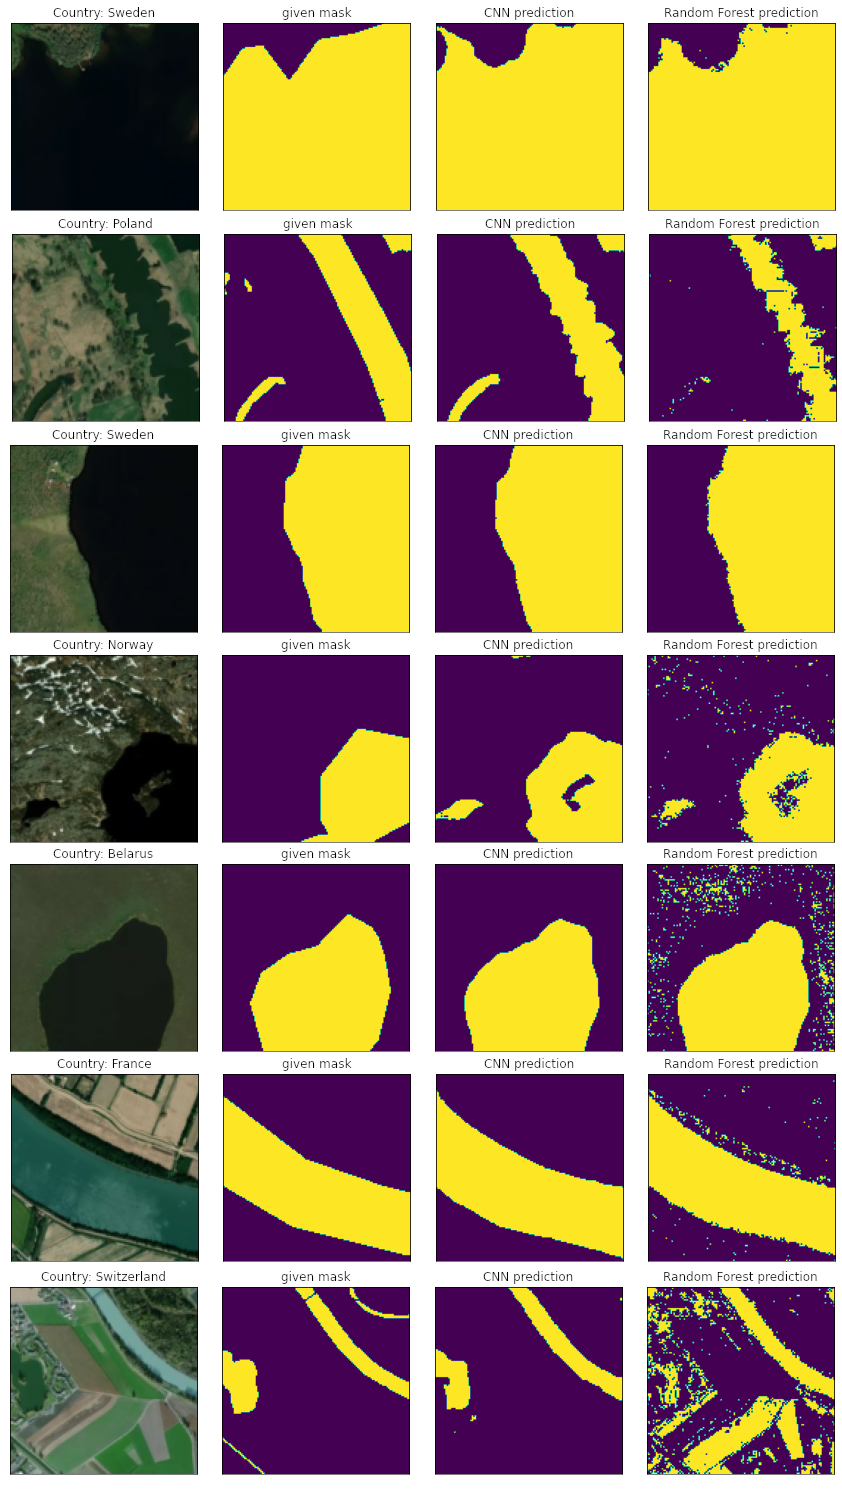
\includegraphics[width=0.8\textwidth]{images/bsp.png}
    \caption{Weitere Beispiele zum Vergleich der Hauptmethode zur Alternativmethode.\\ \copyright Mapbox, \copyright OpenStreetMap}
    \label{fig:bsp}
\end{figure}

\begin{figure}
    \centering
    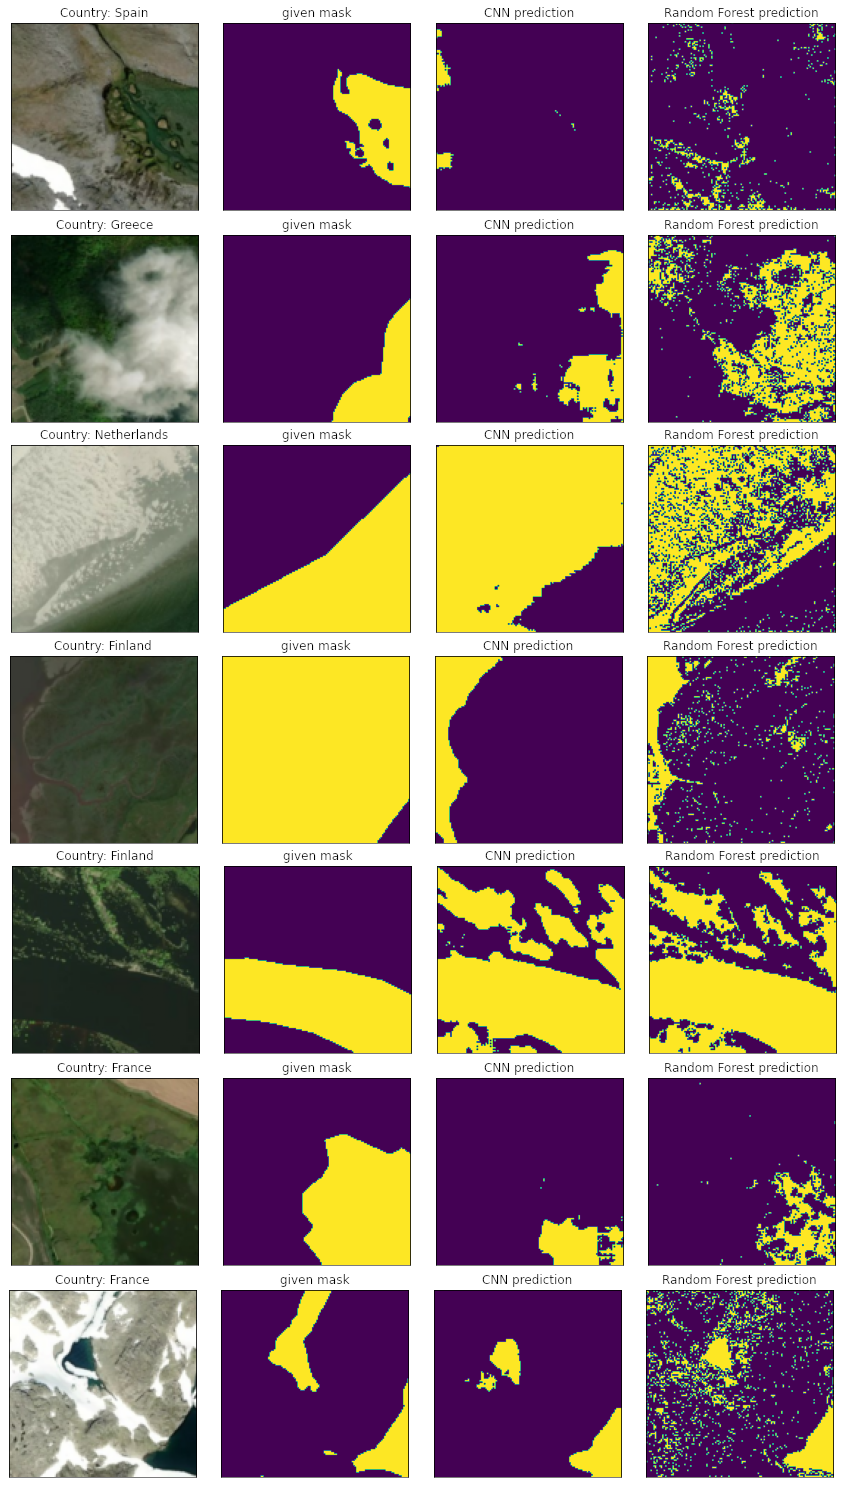
\includegraphics[width=0.8\textwidth]{images/bsp_bad.png}
    \caption{Weitere Beispiele zum Vergleich der Hauptmethode zur Alternativmethode, die schleche Ergebnisse lieferten.\\ \copyright Mapbox, \copyright OpenStreetMap}
    \label{fig:bsp_bad}
\end{figure}
